\documentclass[./../main_file.tex]{subfiles}

\begin{document}
	\subsection{Hệ thống con OnlineLessonSystem}
		\subsubsection{Biểu đồ lớp}
		\begin{figure}[H]
			\centering
			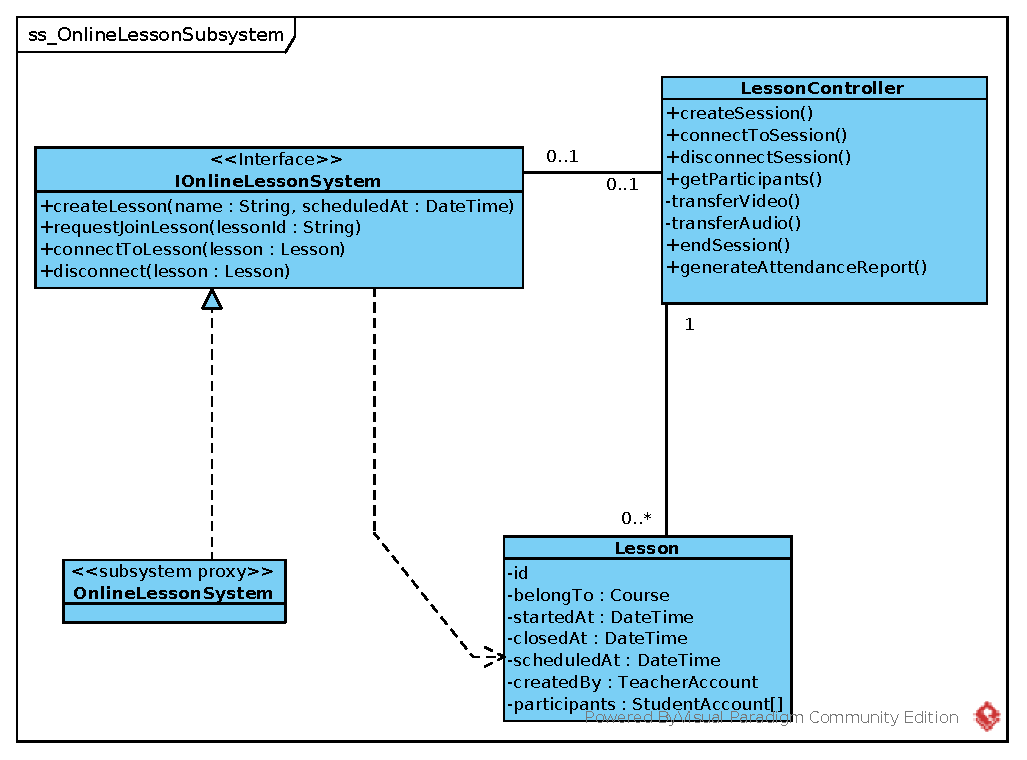
\includegraphics[width=\linewidth]{./images/ss_OnlineLessonSubsystem.eps}
			\caption{Biểu đồ lớp - Hệ thống con OnlineLessonSystem}
		\end{figure}
		\subsubsection{Mô tả hệ thống con}
		\textbf{IOnlineLessonSystem}: Đóng gói các giao tiếp liên quan việc tổ chức và tham gia lớp học trực tuyến.
		\begin{description}
			\item[createLesson(name: String, scheduledAt: DateTime)] Người dùng giáo viên tạo hoặc đặt lịch hẹn cho buổi học trực tuyến.
			\item[requestJoinLesson(lessonId: String)] Người dùng học sinh gửi yêu cầu tham gia vào buổi học trực tuyến.
			\item[connectToLesson(lesson: Lesson)] Người dùng học sinh hoặc giáo viên kết nối tới buổi học trực tuyến để nhận dữ liệu hình ảnh và âm thanh.
			\item[disconnect(lesson: Lesson)] Người dùng ngắt kết nối với buổi học trực tuyến. Nếu người ngắt kết nối là người tạo buổi học, buổi học sẽ được kết thúc.
		\end{description}
		
	\subsection{Hệ thống con AssignmentSystem}
		\subsubsection{Biểu đồ lớp}
		\begin{figure}[H]
			\centering
			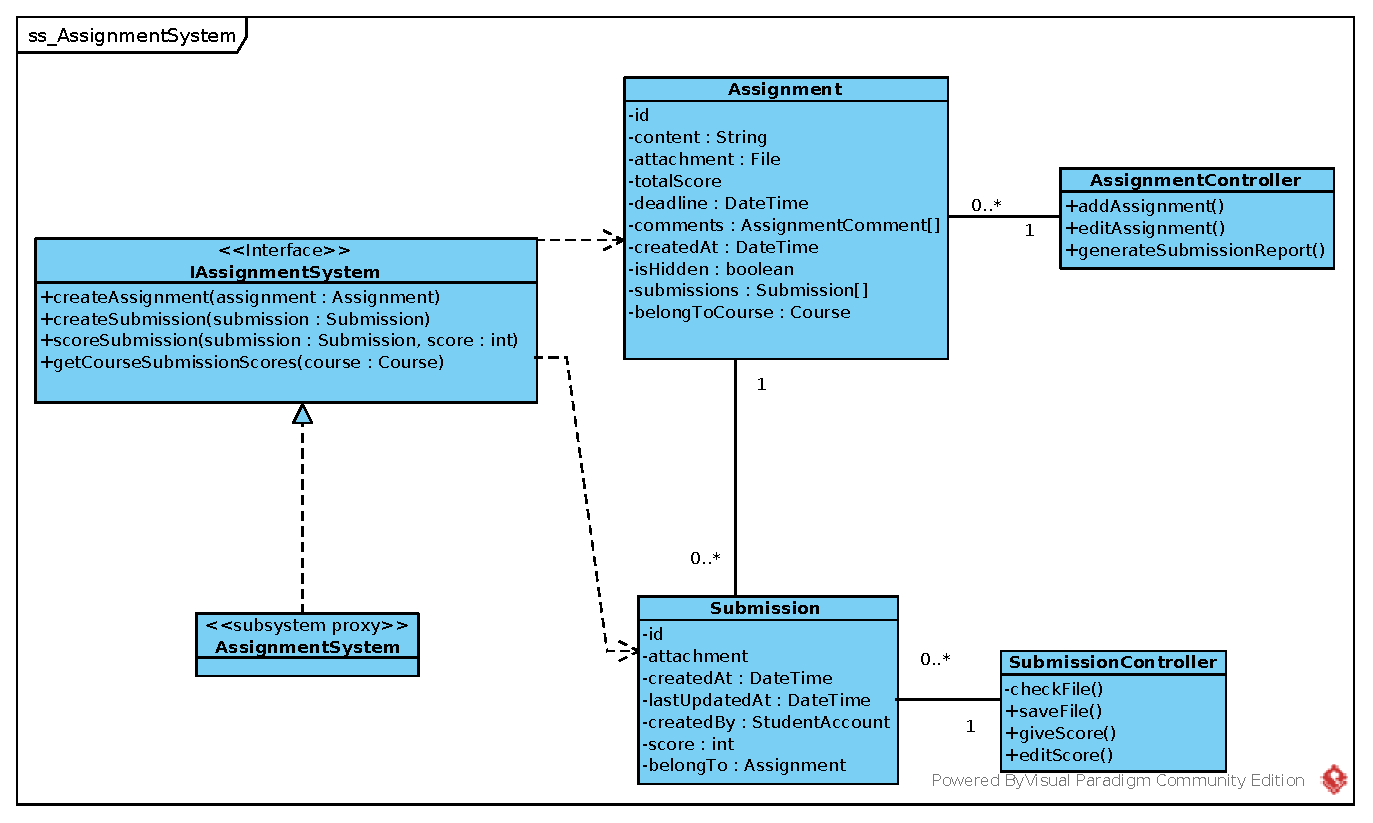
\includegraphics[width=\linewidth]{./images/ss_AssignmentSystem.eps}
			\caption{Biểu đồ lớp - Hệ thống con AssignmentSystem}
		\end{figure}
		\subsubsection{Mô tả hệ thống con}
		\textbf{IAssignmentSystem}: Đóng gói các tính năng gửi, nộp và chấm bài trong khóa học.
		\begin{description}
			\item[createAssignment(assignment : Assignment)] Người dùng giáo viên tạo bài tập (assignment mới) cho lớp học.
			\item[createSubmission(submission : Submission)] Người dùng học sinh tạo bài nộp cho một Assignment trong khóa học.
			\item[scoreSubmission(submission: Submission, score : int)] Người dùng giáo viên thêm điểm cho một bài nộp của học sinh.
			\item[getCourseSubmissionScores(course : Course)] Lấy điểm của tất cả bài nộp trong lớp học.
		\end{description}
		
	\subsection{Hệ thống con NotificationSystem}
		\subsubsection{Biểu đồ lớp}
		\begin{figure}[H]
			\centering
			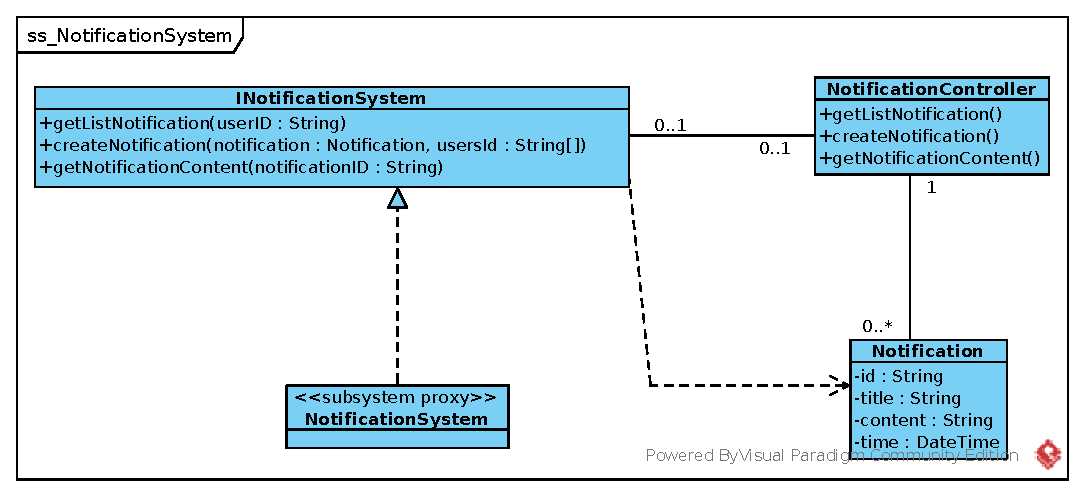
\includegraphics[width=\linewidth]{./images/ss_NotificationSystem.eps}
			\caption{Biểu đồ lớp - Hệ thống con NotificationSystem}
		\end{figure}
		\subsubsection{Mô tả hệ thống con}
		\textbf{INotificationSystem}: Đóng gói các tính năng liên quan đến việc đọc và tạo thông báo tới các người dùng.
		\begin{description}
			\item[getListNotification(userId: String)] lấy về danh sách thông báo của người dùng.
			\item[getNotificationContent(notificationId: String)] lấy về nội dung thông báo.
			\item[createNotification(notification: Notification, userId : String[])] tạo thông báo mới tới các người dùng.
		\end{description}
		
		
	\subsection{Hệ thống con AuthenticationSystem}
		\subsubsection{Biểu đồ lớp}
		\begin{figure}[H]
			\centering
			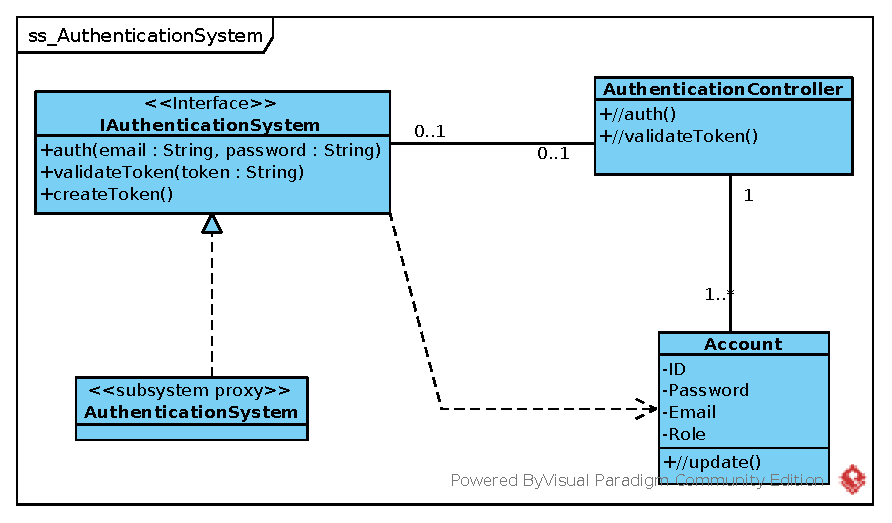
\includegraphics[width=\linewidth]{./images/ss_AuthenticationSystem.eps}
			\caption{Biểu đồ lớp - Hệ thống con AuthenticationSystem}
		\end{figure}
		\subsubsection{Mô tả hệ thống con}
		\textbf{IAuthenticationSystem}: Đóng gói các tính năng đến việc xác thực người dùng và thẻ xác thực người dùng.
		\begin{description}
		\item[auth(email: String, password: String)] xác thực người dùng thông qua việc xác thực email và mật khẩu của người dùng đã cung cấp.
		\item[createToken()] tạo thẻ xác thực người dùng với hệ thống.
		\item[validateToken(token: String)] xác thực thẻ xác thực người dùng.
		\end{description}	
		
	\subsection{Hệ thống con BlogSystem}
		\subsubsection{Biểu đồ lớp}
		\begin{figure}[H]
			\centering
			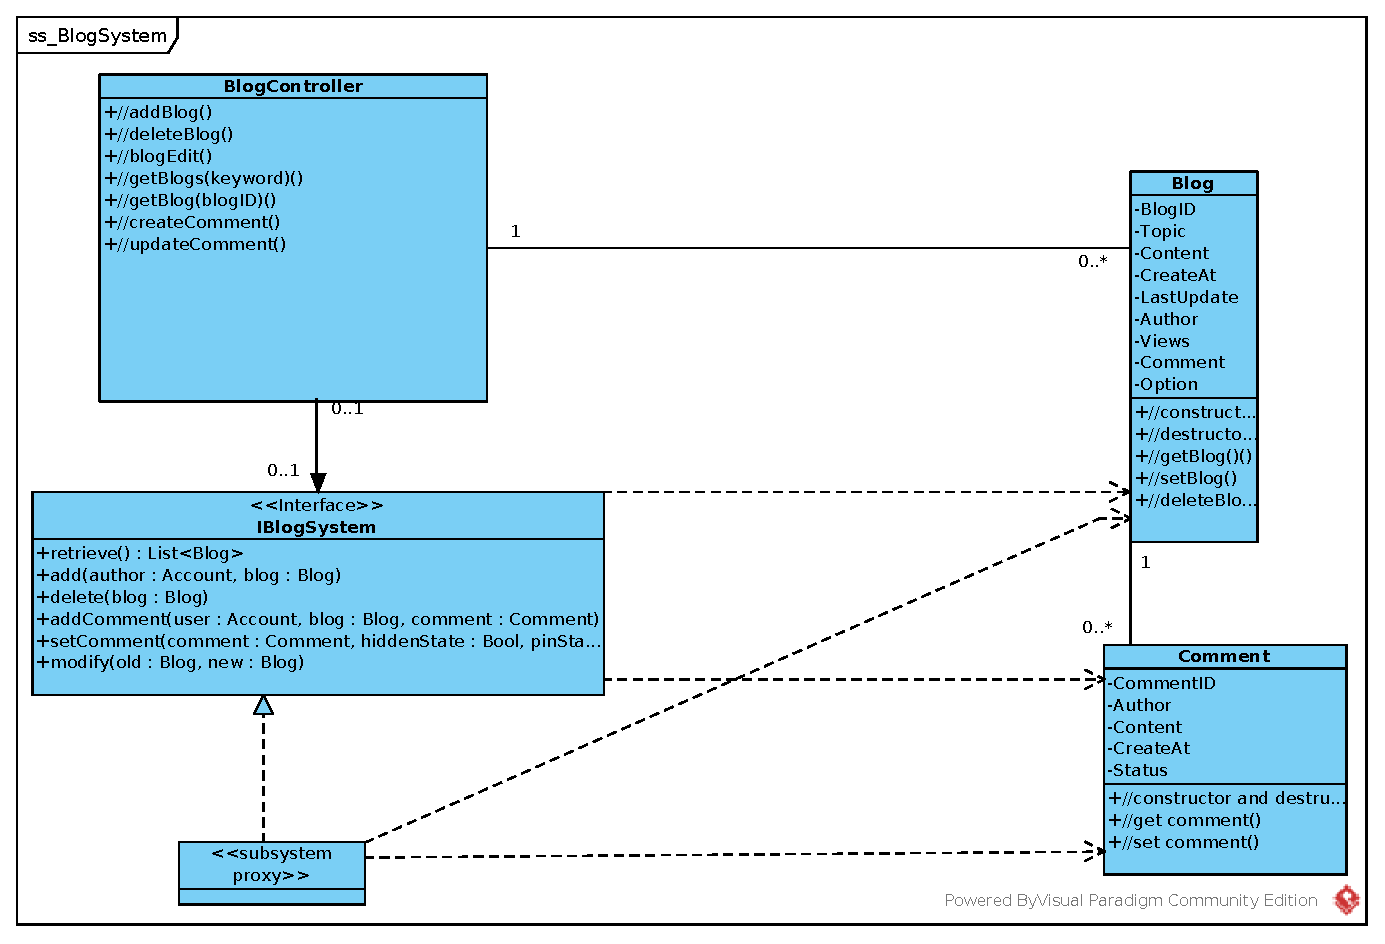
\includegraphics[width=\linewidth]{./images/ss_BlogSystem.eps}
			\caption{Biểu đồ lớp - Hệ thống con BlogSystem}
		\end{figure}
		\subsubsection{Mô tả hệ thống con}
		\textbf{IBlogSystem}: đóng gói các giao tiếp liên quan đến hoạt động đăng bài viết, tương tác với các bài viết giữa những người dùng trên hệ thống
		\begin{description}
			\item[retrieve(): List<Blog>] thu tập tất cả các bài viết được đăng gần nhất trên hệ thống.
			\item[add(author: Account, blog: Blog)] thêm mới bài đăng trên hệ thống.
			\item[delete(blog: Blog)] xóa bài đăng khỏi hệ thống
			\item[addComment(blog:Blog, comment: Comment)] thêm bình luận về bài đăng trên hệ thống.
			\item[setComment(comment: Comment, hiddenState: Bool, pinState: Bool)] cài đặt trạng thái cho bình luận gồm có ẩn bình luận, ghim bình luận.
			\item[modify(old: Blog, new:Blog)] thay đổi các trường nội dung trong bài đăng trên hệ thống.
		\end{description}
		
	\subsection{Hệ thống con MessageSystem}
		\subsubsection{Biểu đồ lớp}
		\begin{figure}[H]
			\centering
			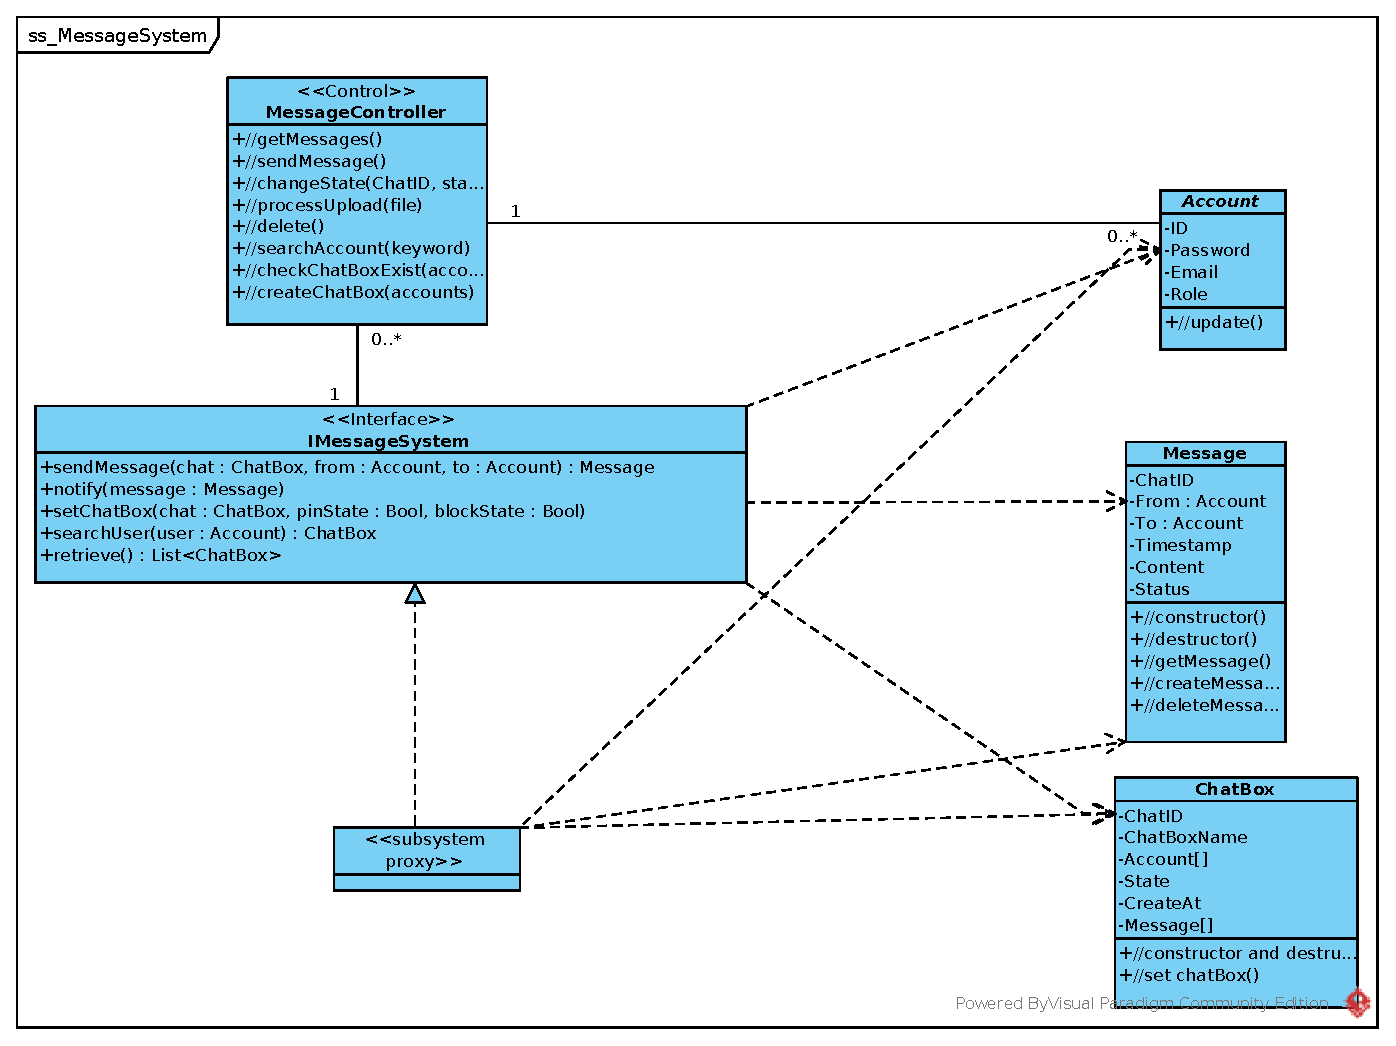
\includegraphics[width=\linewidth]{./images/ss_MessageSystem.eps}
			\caption{Biểu đồ lớp - Hệ thống con MessageSystem}
		\end{figure}
		\subsubsection{Mô tả hệ thống con}
		\textbf{IMessageSystem}: đóng gói các giao tiếp liên quan đến nhắn tin liên lạc giữa những người dùng trên hệ thống
		\begin{description}
			\item[sendMessage(chat: ChatBox, from: Account, to: Account)] Message: Gửi tin nhắn trao đổi, liên lạc giữa những người trong cuộc trò chuyện.
			\item[notify(message: Message)] Thông báo tin nhắn đã được gửi thành công.
			\item[setChatBox(chat: ChatBox, pinState: bool, blockState: bool)] Cài đặt trạng thái cho cuộc trò chuyện gồm có ghim cuộc trò chuyện, chặn cuộc trò chuyện (những người dùng trong cuộc trò chuyện không thể gửi và nhận tin nhắn cho nhau)
			\item[searchUser(user: Account): ChatBox] Tìm kiếm cuộc trò chuyện với người dùng, nếu chưa tồn tại cuộc trò chuyện sẽ tạo một cuộc trò chuyện mới.
			\item[retrieve(): List<ChatBox>] Thu thập để hiển thị các cuộc trò chuyện gần nhất của người dùng trên hệ thống.
		\end{description}
\end{document}